\documentclass[11pt]{beamer}
\usetheme{Madrid}
\usecolortheme{default}

\usepackage{fontspec}
\usepackage{listings}
\usepackage{xcolor}
\usepackage{tikz}
\usetikzlibrary{shapes.symbols, shapes.arrows, positioning, arrows.meta,
                decorations.pathreplacing, fit, backgrounds}

% Font chinh: Arial - co san tren ca Windows lan macOS, du dau tieng Viet
\setmainfont{Arial}
% Font code: DejaVu Sans Mono lay tu chinh TeX Live (goi "dejavu"),
% nen may nao cai TeX cung tim thay - khong phu thuoc font he thong.
%   Muon dung Consolas (chi co tren Windows) thi thay 5 dong duoi bang:
%   \setmonofont{Consolas}
% LUU Y: DejaVu Sans Mono thieu vai chu tieng Viet co dau (o, e, ...),
% vi vay khong go tieng Viet co dau trong \texttt{} va trong lstlisting.
\setmonofont{DejaVuSansMono}[
  Extension=.ttf, UprightFont=*, BoldFont=*-Bold,
  ItalicFont=*-Oblique, BoldItalicFont=*-BoldOblique]

\definecolor{codebg}{RGB}{245,245,245}
% Mau cho cac so do minh hoa
\definecolor{npA}{RGB}{ 77,199,190}
\definecolor{npB}{RGB}{ 26,180,168}
\definecolor{npC}{RGB}{ 58,199,235}
\definecolor{npD}{RGB}{ 42,140,206}
\definecolor{npE}{RGB}{ 22, 71,124}
\definecolor{npWarn}{RGB}{230,120, 40}

\lstset{
  language=Python,
  backgroundcolor=\color{codebg},
  basicstyle=\ttfamily\footnotesize,
  aboveskip=5pt,
  belowskip=5pt,
  keywordstyle=\color{blue}\bfseries,
  commentstyle=\color{gray}\itshape,
  stringstyle=\color{orange},
  showstringspaces=false,
  breaklines=true,
  extendedchars=true,
  inputencoding=utf8,
  frame=single,
  numbers=none,
}

\title{NumPy --- Nền tảng tính toán cho AI}
\subtitle{Thư viện cho Trí tuệ nhân tạo --- Bài 1}
\author{Trình bày: Võ Luyện}
\date{}

\begin{document}

\frame{\titlepage}

\begin{frame}{Nội dung buổi học}
\footnotesize
\begin{columns}[t]
  \begin{column}{0.48\textwidth}
    \tableofcontents[sections={1-7}, hideallsubsections]
  \end{column}
  \begin{column}{0.48\textwidth}
    \tableofcontents[sections={8-14}, hideallsubsections]
  \end{column}
\end{columns}
\end{frame}

% =====================================================================
\section{Vì sao AI cần NumPy?}

\begin{frame}{Dữ liệu trong AI là những con số --- rất nhiều con số}
\begin{itemize}
  \item Một tấm ảnh $224 \times 224$ màu $\to$ $224 \times 224 \times 3 = 150\,528$ con số
  \item Một bảng điểm của 1000 học sinh với 10 môn $\to$ $10\,000$ con số
  \item Một mô hình mạng nơ-ron nhỏ $\to$ hàng triệu tham số cần cập nhật liên tục
\end{itemize}
\pause
\begin{block}{Câu hỏi}
Nếu dùng \texttt{list} của Python thuần và vòng lặp \texttt{for} để xử lý từng con số, chuyện gì xảy ra?
\end{block}
\pause
\begin{alertblock}{Trả lời}
Chương trình chạy \textbf{rất chậm} --- huấn luyện một mô hình có thể mất vài ngày thay vì vài phút.
\end{alertblock}
\end{frame}

\begin{frame}{NumPy là gì?}
\begin{itemize}
  \item \textbf{NumPy} (Numerical Python) --- thư viện tính toán số học nền tảng của Python
  \item Ra đời năm 2006, hiện là "trái tim" của toàn bộ hệ sinh thái khoa học dữ liệu và AI
  \item Cung cấp kiểu dữ liệu \textbf{\texttt{ndarray}} --- mảng nhiều chiều, lưu số hiệu quả
  \item Phần lõi được viết bằng \textbf{C} và Fortran $\to$ nhanh hơn Python thuần hàng chục đến hàng trăm lần
\end{itemize}
\pause
\begin{block}{Ai đang dùng NumPy?}
Pandas, Scikit-learn, Matplotlib, OpenCV, PyTorch, TensorFlow --- tất cả đều xây dựng trên NumPy hoặc dùng chung cách tổ chức dữ liệu của NumPy.
\end{block}
\end{frame}

\begin{frame}{Vị trí của NumPy trong hệ sinh thái AI}
\begin{center}
\begin{tikzpicture}[
    lvl/.style={rounded corners=3pt, draw=none, text=white, minimum height=0.95cm,
                align=center, font=\small\bfseries}
  ]
  \node[lvl, fill=npE, minimum width=9.6cm] (l1) at (0,0)
       {NumPy --- mảng số nhiều chiều \texttt{ndarray}};
  \node[lvl, fill=npD, minimum width=4.7cm] (l2a) at (-2.45,1.15) {Pandas\\ \footnotesize\mdseries dữ liệu dạng bảng};
  \node[lvl, fill=npD, minimum width=4.7cm] (l2b) at (2.45,1.15) {Matplotlib\\ \footnotesize\mdseries vẽ biểu đồ};
  \node[lvl, fill=npC, minimum width=9.6cm] (l3) at (0,2.5)
       {Scikit-learn --- Machine Learning cổ điển};
  \node[lvl, fill=npB, minimum width=9.6cm] (l4) at (0,3.65)
       {PyTorch / TensorFlow --- Deep Learning};
  \node[font=\footnotesize, text width=3cm, align=center] at (0,-1.1)
       {Càng xuống dưới càng nền tảng};
  \draw[-{Stealth[length=3mm]}, thick, npE] (0,-0.85) -- (0,-0.5);
\end{tikzpicture}
\end{center}
\begin{itemize}
  \item Học NumPy tốt $\to$ học các thư viện phía trên nhanh hơn rất nhiều
\end{itemize}
\end{frame}

\begin{frame}[fragile]{So sánh tốc độ: list vs ndarray}
\begin{lstlisting}
import numpy as np, time

n = 1_000_000
list_a = list(range(n))
arr_a  = np.arange(n)

t0 = time.time()
tong1 = sum(x * x for x in list_a)   # Python thuan
t1 = time.time()
tong2 = np.sum(arr_a * arr_a)        # NumPy
t2 = time.time()

print("Python list:", t1 - t0, "giay")
print("NumPy      :", t2 - t1, "giay")
\end{lstlisting}
\begin{block}{Kết quả tham khảo (tùy máy)}
Python list $\approx$ 0.025--0.09 giây; NumPy $\approx$ 0.001--0.002 giây
$\to$ \textbf{nhanh hơn 20--50 lần}
\end{block}
\end{frame}

\begin{frame}{Vì sao NumPy nhanh hơn?}
\begin{center}
\begin{tikzpicture}[
    cell/.style={draw=npE, thick, minimum width=0.85cm, minimum height=0.6cm, font=\small},
    obj/.style={draw=npWarn, thick, rounded corners=2pt, fill=npWarn!12,
                minimum width=0.8cm, minimum height=0.55cm, font=\scriptsize},
    lbl/.style={font=\footnotesize\bfseries}
  ]
  % Python list
  \node[lbl] at (-1.8, 1.55) {Python list};
  \foreach \i in {0,1,2,3} {
    \node[cell, fill=npWarn!25] (p\i) at (\i*0.85, 1.55) {};
  }
  \foreach \i/\v in {0/1, 1/2, 2/3, 3/4} {
    \node[obj] (o\i) at (\i*1.15 - 0.3, 2.7) {int \v};
    \draw[-{Stealth[length=2mm]}, npWarn] (p\i) -- (o\i);
  }
  \node[font=\scriptsize, text width=4.2cm, align=left] at (6.6, 2.1)
       {Mỗi ô chỉ là \textbf{con trỏ} tới một đối tượng Python nằm rải rác trong bộ nhớ.
        Mỗi phép cộng phải: tìm đối tượng $\to$ kiểm tra kiểu $\to$ tính $\to$ tạo đối tượng mới.};

  % NumPy array
  \node[lbl] at (-1.8, -0.55) {NumPy array};
  \foreach \i/\v in {0/1, 1/2, 2/3, 3/4} {
    \node[cell, fill=npA!40] at (\i*0.85, -0.55) {\v};
  }
  \draw[decorate, decoration={brace, amplitude=4pt, mirror}, npE]
       (-0.45,-0.95) -- (3.0,-0.95);
  \node[font=\scriptsize] at (1.3,-1.4) {khối nhớ liên tục, cùng một kiểu};
  \node[font=\scriptsize, text width=4.2cm, align=left] at (6.6, -0.6)
       {Các số nằm \textbf{liền nhau}, cùng kiểu $\to$ vòng lặp chạy trong C, tận dụng cache CPU
        và lệnh xử lý song song (SIMD).};
\end{tikzpicture}
\end{center}
\end{frame}

\begin{frame}{NumPy array khác Python list ở điểm nào?}
\begin{center}
\small
\begin{tabular}{|l|l|l|}
\hline
 & \textbf{Python list} & \textbf{NumPy ndarray} \\
\hline
Kiểu phần tử      & Trộn lẫn tùy ý       & \textbf{Đồng nhất} (int, float, \ldots) \\
Kích thước        & Thay đổi được        & Cố định khi tạo \\
Bộ nhớ            & Nhiều, rải rác       & Ít, liên tục \\
Tốc độ tính toán  & Chậm (vòng lặp)      & Nhanh (chạy trong C) \\
Phép toán số học  & \texttt{[1,2]+[3,4]} $\to$ nối & \texttt{a+b} $\to$ cộng từng phần tử \\
Nhiều chiều       & Phải lồng list       & Hỗ trợ sẵn \\
Hàm toán học      & Phải tự viết         & Có sẵn hàng trăm hàm \\
\hline
\end{tabular}
\end{center}
\begin{alertblock}{Ghi nhớ}
List dùng để chứa \textbf{mọi thứ}. NumPy array dùng để \textbf{tính toán trên số}.
\end{alertblock}
\end{frame}

% =====================================================================
\section{Bắt đầu với NumPy}

\begin{frame}[fragile]{Cài đặt và import}
\textbf{Cài đặt} (chỉ làm một lần, trong Terminal / Command Prompt):
\begin{lstlisting}[language=bash, numbers=none, keywordstyle=\color{black}]
pip install numpy
\end{lstlisting}
Với Google Colab hoặc Anaconda: NumPy đã được cài sẵn.
\vspace{0.3cm}
\textbf{Import} --- quy ước chung của cả thế giới:
\begin{lstlisting}
import numpy as np

print(np.__version__)   # kiem tra phien ban
\end{lstlisting}
\begin{block}{Lưu ý}
Luôn viết \texttt{import numpy as np}. Mọi tài liệu, mọi khóa học, mọi đoạn code trên mạng đều dùng bí danh \texttt{np}.
\end{block}
\end{frame}

\begin{frame}[fragile]{Mảng đầu tiên của bạn}
\begin{lstlisting}
import numpy as np

a = np.array([1, 2, 3, 4, 5])
print(a)          # [1 2 3 4 5]
print(type(a))    # <class 'numpy.ndarray'>

# Phep toan tac dong len TOAN BO mang
print(a + 10)     # [11 12 13 14 15]
print(a * 2)      # [ 2  4  6  8 10]
print(a ** 2)     # [ 1  4  9 16 25]
\end{lstlisting}
\begin{itemize}
  \item Không cần vòng lặp \texttt{for} --- đây gọi là \textbf{vector hóa} (vectorization)
  \item So sánh: với list, \texttt{[1,2,3] * 2} cho \texttt{[1,2,3,1,2,3]} --- hoàn toàn khác!
\end{itemize}
\end{frame}

\begin{frame}{Mảng nhiều chiều --- khái niệm cốt lõi}
\begin{center}
\begin{tikzpicture}[
    cell/.style={draw=npE, minimum width=0.55cm, minimum height=0.48cm, font=\scriptsize},
    npcap/.style={font=\footnotesize\bfseries, align=center}
  ]
  % 1D
  \foreach \i/\v in {0/3, 1/1, 2/4, 3/1} {
    \node[cell, fill=npA!35] at (\i*0.55, 0) {\v};
  }
  \node[npcap] at (0.82, -0.72) {1 chiều (1D)\\ \scriptsize\mdseries vector --- \texttt{shape (4,)}};
  \node[font=\scriptsize] at (0.82, -1.55) {vd: điểm 4 môn học};

  % 2D
  \begin{scope}[xshift=3.8cm]
    \foreach \r in {0,1,2} {
      \foreach \c in {0,1,2,3} {
        \node[cell, fill=npC!35] at (\c*0.55, -\r*0.48) {};
      }
    }
    \node[npcap] at (0.82, -1.8) {2 chiều (2D)\\ \scriptsize\mdseries ma trận --- \texttt{shape (3,4)}};
    \node[font=\scriptsize] at (0.82, -2.6) {vd: bảng điểm 3 HS $\times$ 4 môn};
  \end{scope}

  % 3D
  \begin{scope}[xshift=7.85cm]
    \foreach \lay/\col in {2/npD!20, 1/npD!35, 0/npD!55} {
      \begin{scope}[xshift=\lay*0.22cm, yshift=\lay*0.22cm]
        \foreach \r in {0,1,2} {
          \foreach \c in {0,1,2,3} {
            \node[cell, fill=\col] at (\c*0.55, -\r*0.48) {};
          }
        }
      \end{scope}
    }
    \node[npcap] at (1.0, -1.8) {3 chiều (3D)\\ \scriptsize\mdseries tensor --- \texttt{shape (3,4,3)}};
    \node[font=\scriptsize] at (1.0, -2.6) {vd: ảnh màu cao$\times$rộng$\times$RGB};
  \end{scope}
\end{tikzpicture}
\end{center}
\vspace{0.2cm}
\begin{itemize}
  \item Mọi dữ liệu trong AI --- ảnh, âm thanh, văn bản, bảng số --- đều được đưa về mảng nhiều chiều
\end{itemize}
\end{frame}

\begin{frame}[fragile]{Tạo mảng 2 chiều}
\begin{lstlisting}
diem = np.array([[8.0, 7.5, 9.0],      # hoc sinh 1
                 [6.5, 8.0, 7.0],      # hoc sinh 2
                 [9.0, 9.5, 8.5]])     # hoc sinh 3

print(diem)
print(diem.shape)   # (3, 3)  -> 3 hang, 3 cot
print(diem.ndim)    # 2       -> so chieu
\end{lstlisting}
\begin{itemize}
  \item Mảng 2D được tạo từ \textbf{list của các list}
  \item Mỗi list con là một \textbf{hàng} (row) và phải có \textbf{cùng độ dài}
  \item Quy ước đọc \texttt{shape}: (số hàng, số cột)
\end{itemize}
\end{frame}

% =====================================================================
\section{Các cách tạo mảng}

\begin{frame}[fragile]{Tạo mảng từ giá trị có sẵn}
\begin{lstlisting}
np.zeros(5)          # [0. 0. 0. 0. 0.]
np.zeros((2, 3))     # ma tran 2x3 toan so 0
np.ones((2, 3))      # ma tran 2x3 toan so 1
np.full((2, 3), 7)   # ma tran 2x3 toan so 7
np.eye(3)            # ma tran don vi 3x3 (duong cheo = 1)
np.empty((2, 2))     # chua khoi tao - gia tri rac, rat nhanh
\end{lstlisting}
\begin{itemize}
  \item Chú ý \textbf{dấu ngoặc kép}: \texttt{np.zeros((2, 3))} --- hình dạng là một \textbf{tuple}
  \item \texttt{np.zeros} rất hay dùng để khởi tạo trọng số hoặc bộ đếm trong AI
\end{itemize}
\begin{alertblock}{Lỗi thường gặp}
\texttt{np.zeros(2, 3)} $\to$ báo lỗi. Tham số thứ hai là \texttt{dtype}, không phải số cột!
\end{alertblock}
\end{frame}

\begin{frame}[fragile]{Tạo dãy số: arange và linspace}
\begin{lstlisting}
np.arange(5)             # [0 1 2 3 4]
np.arange(2, 10)         # [2 3 4 5 6 7 8 9]
np.arange(0, 10, 2)      # [0 2 4 6 8]      buoc nhay = 2
np.arange(0, 1, 0.25)    # [0.   0.25 0.5  0.75]

np.linspace(0, 1, 5)     # [0.   0.25 0.5  0.75 1.  ]
np.linspace(0, 10, 3)    # [ 0.  5. 10.]
\end{lstlisting}
\begin{center}
\small
\begin{tabular}{|l|l|l|}
\hline
 & \textbf{Bạn chỉ định} & \textbf{Điểm cuối} \\
\hline
\texttt{np.arange(a, b, buoc)} & bước nhảy & \textbf{không} lấy \texttt{b} \\
\texttt{np.linspace(a, b, n)}  & số phần tử & \textbf{có} lấy \texttt{b} \\
\hline
\end{tabular}
\end{center}
\begin{itemize}
  \item Vẽ đồ thị hàm số $\to$ dùng \texttt{linspace}; tạo chỉ số đếm $\to$ dùng \texttt{arange}
\end{itemize}
\end{frame}

\begin{frame}[fragile]{Tạo mảng ngẫu nhiên}
\begin{lstlisting}
rng = np.random.default_rng(42)   # 42 la "hat giong" (seed)

rng.random(5)             # 5 so thuc ngau nhien trong [0, 1)
rng.random((2, 3))        # ma tran 2x3 so thuc ngau nhien
rng.integers(1, 7, 10)    # 10 so nguyen 1..6 (gieo xuc xac)
rng.normal(0, 1, 5)      # 5 so phan phoi chuan (mean 0, std 1)
\end{lstlisting}
\begin{block}{Vì sao cần seed?}
Đặt seed $\to$ lần chạy nào cũng cho \textbf{cùng một kết quả} $\to$ thí nghiệm AI có thể \textbf{lặp lại được} (reproducible). Đây là nguyên tắc bắt buộc khi làm nghiên cứu.
\end{block}
\begin{itemize}
  \item Cách cũ (vẫn gặp nhiều trong tài liệu): \texttt{np.random.seed(42)} rồi \texttt{np.random.rand(5)}
\end{itemize}
\end{frame}

% =====================================================================
\section{Thuộc tính và kiểu dữ liệu}

\begin{frame}[fragile]{Các thuộc tính quan trọng của mảng}
\begin{lstlisting}
a = np.array([[1, 2, 3],
              [4, 5, 6]])

print(a.shape)      # (2, 3)   hinh dang: 2 hang, 3 cot
print(a.ndim)       # 2        so chieu
print(a.size)       # 6        tong so phan tu
print(a.dtype)      # int64    kieu du lieu cua phan tu
print(a.itemsize)   # 8        so byte moi phan tu
print(a.nbytes)     # 48       tong so byte = size * itemsize
\end{lstlisting}
\begin{alertblock}{Thói quen tốt số 1 khi làm AI}
Gặp lỗi hay nghi ngờ $\to$ \texttt{print(x.shape)} \textbf{ngay lập tức}. Hơn 80\% lỗi khi lập trình AI là do \textbf{sai hình dạng mảng}.
\end{alertblock}
\end{frame}

\begin{frame}[fragile]{Kiểu dữ liệu (dtype)}
\begin{lstlisting}
np.array([1, 2, 3]).dtype         # int64  (Windows cu: int32)
np.array([1.0, 2.0]).dtype         # float64
np.array([1, 2], dtype=np.float32) # ep kieu ngay khi tao

a = np.array([1.7, 2.3, 3.9])
b = a.astype(int)      # [1 2 3] - CAT phan thap phan
c = a.astype(np.float32)
\end{lstlisting}
\begin{center}
\small
\begin{tabular}{|l|l|l|}
\hline
\textbf{Kiểu} & \textbf{Bộ nhớ} & \textbf{Dùng khi} \\
\hline
\texttt{uint8}   & 1 byte & Ảnh (giá trị 0--255) \\
\texttt{int32/int64} & 4/8 byte & Nhãn, chỉ số, số đếm \\
\texttt{float32} & 4 byte & \textbf{Chuẩn của Deep Learning} \\
\texttt{float64} & 8 byte & Mặc định của NumPy, độ chính xác cao \\
\texttt{bool}    & 1 byte & Mặt nạ lọc dữ liệu \\
\hline
\end{tabular}
\end{center}
\end{frame}

\begin{frame}[fragile]{Cẩn thận với kiểu số nguyên}
\begin{lstlisting}
a = np.array([250, 251, 252], dtype=np.uint8)
print(a + 10)      # [4 5 6]  ??? -- TRAN SO (overflow)!
# uint8 chi chua duoc 0..255, 260 quay vong ve 4

b = np.array([1, 2, 3])
b[0] = 3.9
print(b)           # [3 2 3]  -- bi cat thanh so nguyen
\end{lstlisting}
\begin{alertblock}{Quy tắc an toàn khi làm AI}
Trước khi tính toán trên ảnh, luôn đổi sang số thực:
\texttt{img = img.astype(np.float32) / 255.0}
\end{alertblock}
\end{frame}

% =====================================================================
\section{Truy cập phần tử: indexing và slicing}

\begin{frame}[fragile]{Indexing và slicing mảng 1 chiều}
\begin{lstlisting}
a = np.array([10, 20, 30, 40, 50, 60])

a[0]        # 10   phan tu dau tien
a[-1]       # 60   phan tu cuoi cung
a[1:4]      # [20 30 40]   tu chi so 1 den 3
a[:3]       # [10 20 30]   3 phan tu dau
a[3:]       # [40 50 60]   tu chi so 3 den het
a[::2]      # [10 30 50]   cach 1 lay 1
a[::-1]     # [60 50 40 30 20 10]   dao nguoc
\end{lstlisting}
\begin{itemize}
  \item Cú pháp giống hệt list của Python: \texttt{a[start : stop : step]} --- bắt đầu, kết thúc, bước nhảy
  \item Luôn nhớ: chỉ số bắt đầu từ \textbf{0}, và \textbf{không} lấy phần tử ở vị trí \texttt{stop}
\end{itemize}
\end{frame}

\begin{frame}[fragile]{Indexing mảng 2 chiều}
\begin{lstlisting}
a = np.array([[ 1,  2,  3,  4],
              [ 5,  6,  7,  8],
              [ 9, 10, 11, 12]])

a[1, 2]       # 7      hang 1, cot 2
a[1][2]       # 7     cach viet cua list - cham, TRANH DUNG
a[0]          # [1 2 3 4]        toan bo hang 0
a[:, 1]       # [2 6 10]         toan bo cot 1
a[0:2, 1:3]   # [[2 3], [6 7]]   mang con 2x2
a[-1, -1]     # 12               phan tu goc duoi phai
\end{lstlisting}
\begin{block}{Cách đọc}
Dấu phẩy ngăn cách các chiều: \texttt{a[i, j]} --- hàng \texttt{i}, cột \texttt{j}. Dấu hai chấm \texttt{:} nghĩa là "lấy tất cả".
\end{block}
\end{frame}

\begin{frame}{Minh họa slicing 2 chiều}
\begin{center}
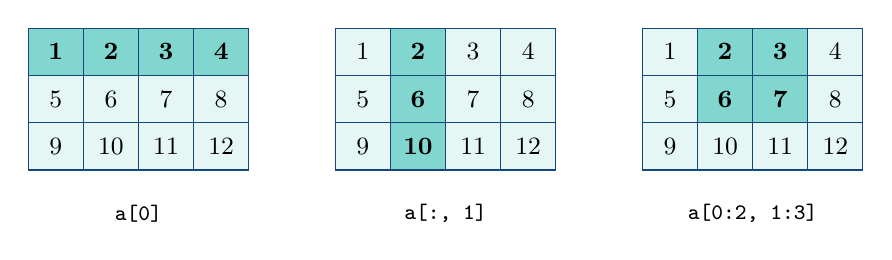
\begin{tikzpicture}[
    cell/.style={draw=npE, minimum width=0.7cm, minimum height=0.6cm, font=\small},
    hl/.style={cell, fill=npB!55, font=\small\bfseries},
    ttl/.style={font=\footnotesize\ttfamily}
  ]
  % a[0]
  \foreach \r in {0,1,2} \foreach \c in {0,1,2,3} {
    \pgfmathtruncatemacro{\v}{\r*4 + \c + 1}
    \pgfmathtruncatemacro{\hit}{(\r==0) ? 1 : 0}
    \ifnum\hit=1
      \node[hl] at (\c*0.7, -\r*0.6) {\v};
    \else
      \node[cell, fill=npA!15] at (\c*0.7, -\r*0.6) {\v};
    \fi
  }
  \node[ttl] at (1.05, -2.05) {a[0]};

  % a[:, 1]
  \begin{scope}[xshift=3.9cm]
    \foreach \r in {0,1,2} \foreach \c in {0,1,2,3} {
      \pgfmathtruncatemacro{\v}{\r*4 + \c + 1}
      \pgfmathtruncatemacro{\hit}{(\c==1) ? 1 : 0}
      \ifnum\hit=1
        \node[hl] at (\c*0.7, -\r*0.6) {\v};
      \else
        \node[cell, fill=npA!15] at (\c*0.7, -\r*0.6) {\v};
      \fi
    }
    \node[ttl] at (1.05, -2.05) {a[:, 1]};
  \end{scope}

  % a[0:2, 1:3]
  \begin{scope}[xshift=7.8cm]
    \foreach \r in {0,1,2} \foreach \c in {0,1,2,3} {
      \pgfmathtruncatemacro{\v}{\r*4 + \c + 1}
      \pgfmathtruncatemacro{\hit}{(\r<2 && \c>0 && \c<3) ? 1 : 0}
      \ifnum\hit=1
        \node[hl] at (\c*0.7, -\r*0.6) {\v};
      \else
        \node[cell, fill=npA!15] at (\c*0.7, -\r*0.6) {\v};
      \fi
    }
    \node[ttl] at (1.05, -2.05) {a[0:2, 1:3]};
  \end{scope}
\end{tikzpicture}
\end{center}
\end{frame}

\begin{frame}[fragile]{Lọc dữ liệu bằng điều kiện (boolean masking)}
\begin{lstlisting}
diem = np.array([8.5, 4.0, 7.0, 9.5, 5.5, 3.0])

mask = diem >= 5
print(mask)          # [True False True True True False]
print(diem[mask])    # [8.5 7.  9.5 5.5]   chi lay diem >= 5
print(diem[diem >= 5])            # viet gon, rat pho bien

print(np.sum(diem >= 5))          # 4  - dem so hoc sinh dat
print(np.mean(diem >= 5))         # 0.666... - ti le dat

# Ket hop nhieu dieu kien: dung & (va), | (hoac), ~ (phu dinh)
print(diem[(diem >= 5) & (diem < 9)])   # [8.5 7.  5.5]
\end{lstlisting}
\begin{alertblock}{Chú ý}
Dùng \texttt{\&}, \texttt{|} chứ \textbf{không} dùng \texttt{and}, \texttt{or}. Và \textbf{bắt buộc} có dấu ngoặc quanh mỗi điều kiện.
\end{alertblock}
\end{frame}

\begin{frame}[fragile]{Fancy indexing và np.where}
\textbf{Lấy nhiều phần tử theo danh sách chỉ số:}
\begin{lstlisting}
a = np.array([10, 20, 30, 40, 50])
a[[0, 2, 4]]        # [10 30 50]
a[[4, 4, 0]]        # [50 50 10]  - lap lai duoc, thu tu tuy y
\end{lstlisting}
\textbf{\texttt{np.where} --- "nếu \ldots thì \ldots ngược lại":}
\begin{lstlisting}
diem = np.array([8.5, 4.0, 7.0, 3.0])

np.where(diem >= 5, 1, 0)      # [1 0 1 0] - gan nhan Dat/Truot
np.where(diem >= 5, diem, 0)    # [8.5 0. 7. 0.] - truot -> 0
np.where(diem >= 5)             # (array([0, 2]),) - vi tri
\end{lstlisting}
\begin{itemize}
  \item \texttt{np.where} chính là cách viết \texttt{if--else} \textbf{cho cả mảng}, không cần vòng lặp
\end{itemize}
\end{frame}

% =====================================================================
\section{View và Copy --- cái bẫy kinh điển}

\begin{frame}[fragile]{Slicing tạo ra "view", không phải bản sao}
\begin{lstlisting}
a = np.array([1, 2, 3, 4, 5])
b = a[1:4]       # b la VIEW - nhin vao cung vung nho voi a
b[0] = 99

print(b)          # [99  3  4]
print(a)          # [ 1 99  3  4  5]   <-- a CUNG BI DOI!
\end{lstlisting}
\pause
\textbf{Muốn có bản sao độc lập $\to$ dùng \texttt{.copy()}:}
\begin{lstlisting}
c = a[1:4].copy()
c[0] = 0
print(a)          # [ 1 99  3  4  5]   <-- a khong doi
\end{lstlisting}
\begin{block}{Vì sao NumPy làm vậy?}
Để \textbf{tiết kiệm bộ nhớ} --- cắt một mảng 1GB mà phải sao chép thì rất tốn kém.
\end{block}
\end{frame}

\begin{frame}[fragile]{Khi nào là view, khi nào là copy?}
\begin{center}
\small
\begin{tabular}{|l|l|}
\hline
\textbf{Thao tác} & \textbf{Kết quả} \\
\hline
\texttt{b = a[1:4]}          & \textbf{View} --- dùng chung bộ nhớ \\
\texttt{b = a[a > 5]}        & Copy (boolean masking) \\
\texttt{b = a[[0, 2]]}       & Copy (fancy indexing) \\
\texttt{b = a.reshape(2, 3)} & \textbf{View} (nếu có thể) \\
\texttt{b = a.T}             & \textbf{View} \\
\texttt{b = a.copy()}        & Copy \\
\texttt{b = a + 0}           & Copy (mảng mới từ phép toán) \\
\hline
\end{tabular}
\end{center}
\begin{lstlisting}
b = a[1:4]
print(b.base is a)   # True  -> b la view cua a
\end{lstlisting}
\begin{alertblock}{Quy tắc vàng cho người mới}
Nếu bạn định \textbf{sửa} dữ liệu và \textbf{không} muốn ảnh hưởng mảng gốc $\to$ luôn gọi \texttt{.copy()}.
\end{alertblock}
\end{frame}

% =====================================================================
\section{Vector hóa --- tính toán không cần vòng lặp}

\begin{frame}[fragile]{Phép toán trên từng phần tử (element-wise)}
\begin{lstlisting}
a = np.array([1, 2, 3, 4])
b = np.array([10, 20, 30, 40])

a + b       # [11 22 33 44]
b - a       # [ 9 18 27 36]
a * b       # [ 10  40  90 160]  nhan TUNG PHAN TU
b / a       # [10. 10. 10. 10.]
a ** 2      # [ 1  4  9 16]
b % 3       # [1 2 0 1]

a > 2       # [False False  True  True]
\end{lstlisting}
\begin{itemize}
  \item Hai mảng phải có \textbf{cùng hình dạng} (hoặc tuân theo quy tắc broadcasting ở phần sau)
  \item Kết quả luôn là một mảng \textbf{mới}, cùng hình dạng
\end{itemize}
\end{frame}

\begin{frame}[fragile]{Các hàm toán học có sẵn (universal functions)}
\begin{lstlisting}
a = np.array([1, 4, 9, 16])

np.sqrt(a)      # [1. 2. 3. 4.]      can bac hai
np.exp(a)       # e^a                 ham mu
np.log(a)       # ln(a)               logarit tu nhien
np.abs(-a)      # gia tri tuyet doi
np.round(np.array([1.234, 5.678]), 1)   # [1.2 5.7]

x = np.linspace(0, np.pi, 5)
np.sin(x)       # ham luong giac
np.maximum(a, 5)   # [ 5  5  9 16]  so sanh tung phan tu voi 5
\end{lstlisting}
\begin{block}{Vì sao quan trọng với AI?}
Các hàm kích hoạt (activation) của mạng nơ-ron --- sigmoid, tanh, ReLU, softmax --- đều được viết chỉ bằng vài hàm này.
\end{block}
\end{frame}

\begin{frame}[fragile]{Vector hóa: viết lại vòng lặp cho gọn và nhanh}
\textbf{Cách viết của người mới (chậm):}
\begin{lstlisting}
ket_qua = []
for i in range(len(diem)):
    ket_qua.append(diem[i] * 2 + 1)
ket_qua = np.array(ket_qua)
\end{lstlisting}
\textbf{Cách viết NumPy (nhanh hơn hàng chục lần):}
\begin{lstlisting}
ket_qua = diem * 2 + 1
\end{lstlisting}
\pause
\begin{alertblock}{Nguyên tắc số 1 khi lập trình AI với NumPy}
Thấy vòng lặp \texttt{for} chạy trên từng phần tử của mảng $\to$ hãy nghĩ cách viết lại bằng phép toán trên cả mảng.
\end{alertblock}
\end{frame}

% =====================================================================
\section{Broadcasting}

\begin{frame}[fragile]{Broadcasting --- khi hai mảng khác hình dạng}
\begin{lstlisting}
a = np.array([1, 2, 3])
print(a + 10)      # [11 12 13]  - so 10 duoc "phat" ra ca mang

diem = np.array([[8.0, 7.0, 9.0],     # 3 hoc sinh
                 [6.0, 8.5, 7.5],     # x 3 mon
                 [9.0, 9.0, 8.0]])
he_so = np.array([2, 1, 1])       # Toan he so 2, Ly 1, Hoa 1

print(diem * he_so)    # moi HANG deu duoc nhan voi he_so
\end{lstlisting}
\begin{block}{Broadcasting là gì?}
NumPy tự động "kéo giãn" mảng nhỏ hơn cho khớp hình dạng mảng lớn --- \textbf{không tốn thêm bộ nhớ}, không cần vòng lặp.
\end{block}
\end{frame}

\begin{frame}{Minh họa broadcasting}
\begin{center}
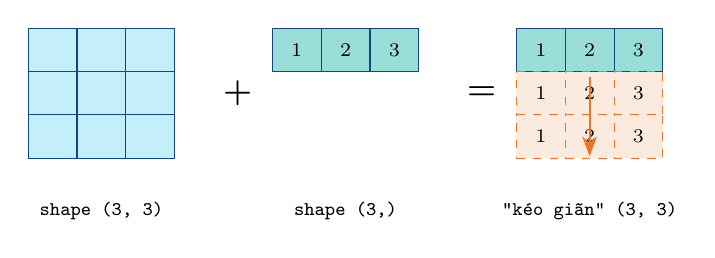
\begin{tikzpicture}[
    cell/.style={draw=npE, minimum width=0.62cm, minimum height=0.55cm, font=\scriptsize},
    ghost/.style={cell, fill=npWarn!15, dashed, draw=npWarn},
    op/.style={font=\large\bfseries}
  ]
  % matrix 3x3
  \foreach \r in {0,1,2} \foreach \c in {0,1,2} {
    \node[cell, fill=npC!30] at (\c*0.62, -\r*0.55) {};
  }
  \node[font=\scriptsize\ttfamily] at (0.62, -2.05) {shape (3, 3)};

  \node[op] at (2.35, -0.55) {+};

  % vector shape (3,)
  \foreach \c/\v in {0/1, 1/2, 2/3} {
    \node[cell, fill=npB!45] at (3.1 + \c*0.62, 0) {\v};
  }
  \node[font=\scriptsize\ttfamily] at (3.72, -2.05) {shape (3,)};

  \node[op] at (5.45, -0.55) {=};

  % broadcast result
  \begin{scope}[xshift=6.2cm]
    \foreach \r in {0,1,2} \foreach \c/\v in {0/1, 1/2, 2/3} {
      \ifnum\r=0
        \node[cell, fill=npB!45] at (\c*0.62, -\r*0.55) {\v};
      \else
        \node[ghost] at (\c*0.62, -\r*0.55) {\v};
      \fi
    }
    \node[font=\scriptsize\ttfamily] at (0.62, -2.05) {"kéo giãn" (3, 3)};
  \end{scope}
  \draw[-{Stealth[length=2.5mm]}, npWarn, thick] (6.82,-0.35) -- (6.82,-1.35);
\end{tikzpicture}
\end{center}
\vspace{0.15cm}
\begin{itemize}
  \item Hàng \texttt{[1 2 3]} được lặp lại cho \textbf{mọi hàng} của ma trận
  \item Việc "kéo giãn" chỉ là \textbf{khái niệm} --- NumPy không thực sự tạo bản sao trong bộ nhớ
\end{itemize}
\end{frame}

\begin{frame}[fragile]{Quy tắc broadcasting}
So sánh hình dạng \textbf{từ phải sang trái}. Hai chiều tương thích khi:
\begin{enumerate}
  \item Chúng \textbf{bằng nhau}, hoặc
  \item Một trong hai \textbf{bằng 1}, hoặc
  \item Một mảng \textbf{không có} chiều đó (được coi như bằng 1)
\end{enumerate}
\vspace{0.2cm}
\begin{center}
\small
\begin{tabular}{|l|l|l|}
\hline
\textbf{Hình dạng A} & \textbf{Hình dạng B} & \textbf{Kết quả} \\
\hline
\texttt{(3, 4)} & \texttt{(4,)}   & \texttt{(3, 4)} --- OK \\
\texttt{(3, 4)} & \texttt{(3, 1)} & \texttt{(3, 4)} --- OK \\
\texttt{(3, 1)} & \texttt{(1, 4)} & \texttt{(3, 4)} --- OK, giãn cả hai \\
\texttt{(3, 4)} & \texttt{(3,)}   & \textcolor{red}{Lỗi} --- 4 và 3 không khớp \\
\hline
\end{tabular}
\end{center}
\begin{lstlisting}
ValueError: operands could not be broadcast together
            with shapes (3,4) (3,)
\end{lstlisting}
\end{frame}

\begin{frame}[fragile]{Ứng dụng broadcasting: chuẩn hóa dữ liệu}
Chuẩn hóa (normalization) là bước \textbf{bắt buộc} trước khi huấn luyện mô hình:
\begin{lstlisting}
# X: 100 mau du lieu, moi mau co 4 dac trung (features)
X = rng.normal(50, 10, size=(100, 4))

mean = X.mean(axis=0)   # shape (4,)  - trung binh TUNG COT
std  = X.std(axis=0)    # shape (4,)  - do lech chuan tung cot

X_chuan = (X - mean) / std     # broadcasting: (100,4) voi (4,)

print(X_chuan.mean(axis=0))    # ~ [0. 0. 0. 0.]
print(X_chuan.std(axis=0))     # ~ [1. 1. 1. 1.]
\end{lstlisting}
\begin{itemize}
  \item Chỉ \textbf{một dòng} thay cho hai vòng lặp lồng nhau và 400 phép tính thủ công
  \item Đây gọi là chuẩn hóa \textbf{z-score} --- công thức $z = (x - \mu) / \sigma$
\end{itemize}
\end{frame}

% =====================================================================
\section{Hàm thống kê và khái niệm axis}

\begin{frame}[fragile]{Các hàm tổng hợp}
\begin{lstlisting}
a = np.array([3, 1, 4, 1, 5, 9, 2, 6])

a.sum()       # 31    tong
a.mean()      # 3.875 trung binh
a.min()       # 1     gia tri nho nhat
a.max()       # 9     gia tri lon nhat
a.std()       # do lech chuan
a.argmin()    # 1     VI TRI cua gia tri nho nhat
a.argmax()    # 5     VI TRI cua gia tri lon nhat
np.median(a)  # 3.5   trung vi
a.cumsum()    # [ 3  4  8  9 14 23 25 31]  tong tich luy
\end{lstlisting}
\begin{block}{\texttt{argmax} --- hàm quan trọng bậc nhất trong AI}
Mô hình phân loại trả về xác suất cho từng lớp; \texttt{argmax} cho biết \textbf{lớp nào có xác suất cao nhất} $\to$ đó là dự đoán của mô hình.
\end{block}
\end{frame}

\begin{frame}{axis --- chiều nào bị "gộp lại"?}
\begin{center}
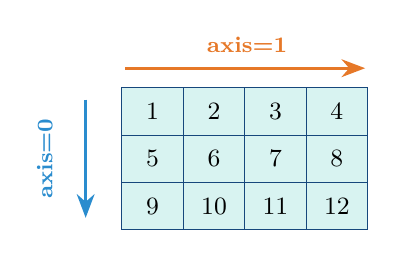
\begin{tikzpicture}[
    cell/.style={draw=npE, minimum width=0.78cm, minimum height=0.6cm, font=\small}
  ]
  \foreach \r in {0,1,2} \foreach \c in {0,1,2,3} {
    \pgfmathtruncatemacro{\v}{\r*4 + \c + 1}
    \node[cell, fill=npA!22] at (\c*0.78, -\r*0.6) {\v};
  }
  % axis 0 arrow (down)
  \draw[-{Stealth[length=3mm]}, very thick, npD] (-0.85, 0.15) -- (-0.85, -1.35);
  \node[npD, font=\footnotesize\bfseries, rotate=90, anchor=south] at (-1.15, -0.6) {axis=0};
  % axis 1 arrow (right)
  \draw[-{Stealth[length=3mm]}, very thick, npWarn] (-0.35, 0.55) -- (2.7, 0.55);
  \node[npWarn, font=\footnotesize\bfseries] at (1.2, 0.85) {axis=1};
\end{tikzpicture}
\end{center}
\begin{center}
\small
\begin{tabular}{|l|l|l|}
\hline
\textbf{Lệnh} & \textbf{Ý nghĩa} & \textbf{Kết quả} \\
\hline
\texttt{a.sum()}       & tổng tất cả              & \texttt{78} \\
\texttt{a.sum(axis=0)} & gộp các \textbf{hàng} $\to$ tổng mỗi \textbf{cột} & \texttt{[15 18 21 24]} \\
\texttt{a.sum(axis=1)} & gộp các \textbf{cột} $\to$ tổng mỗi \textbf{hàng}  & \texttt{[10 26 42]} \\
\hline
\end{tabular}
\end{center}
\begin{alertblock}{Mẹo nhớ}
\texttt{axis=k} nghĩa là "chiều thứ $k$ \textbf{biến mất}". Mảng \texttt{(3,4)} với \texttt{axis=0} $\to$ còn lại \texttt{(4,)}.
\end{alertblock}
\end{frame}

\begin{frame}[fragile]{Ví dụ thực tế với axis}
\begin{lstlisting}
# 4 hoc sinh x 3 mon (Toan, Ly, Hoa)
diem = np.array([[8.0, 7.0, 9.0],
                 [6.0, 8.5, 7.5],
                 [9.0, 9.0, 8.0],
                 [5.0, 6.0, 6.5]])

diem.mean(axis=1)     # DTB cua tung HOC SINH  -> 4 gia tri
diem.mean(axis=0)     # DTB cua tung MON       -> 3 gia tri
diem.max(axis=0)      # diem cao nhat moi mon
diem.argmax(axis=0)   # hoc sinh gioi nhat moi mon (chi so)

# Giu nguyen so chieu de tien broadcasting
tb = diem.mean(axis=1, keepdims=True)   # shape (4,1) ko (4,)
print(diem - tb)      # do lech so voi DTB cua chinh minh
\end{lstlisting}
\end{frame}

% =====================================================================
\section{Biến đổi hình dạng và ghép mảng}

\begin{frame}[fragile]{reshape --- thay đổi hình dạng}
\begin{lstlisting}
a = np.arange(12)          # [0 1 2 ... 11]   shape (12,)

b = a.reshape(3, 4)        # 3 hang, 4 cot
c = a.reshape(4, 3)        # 4 hang, 3 cot
d = a.reshape(2, 2, 3)     # mang 3 chieu
e = a.reshape(3, -1)       # -1 = "tu tinh giup toi" -> (3, 4)

print(b.ravel())          # [0 1 ... 11]  tra ve 1 chieu (view)
print(b.flatten())         # giong ravel nhung tra ve BAN SAO
\end{lstlisting}
\begin{itemize}
  \item Số phần tử phải \textbf{không đổi}: $3 \times 4 = 12$ (được), $5 \times 3 = 15$ (lỗi)
  \item \texttt{-1} cực kỳ hay dùng: \texttt{X.reshape(-1, 784)} --- "gộp ảnh thành vector 784 chiều, số ảnh tự tính"
\end{itemize}
\begin{alertblock}{Lỗi thường gặp}
\texttt{ValueError: cannot reshape array of size 12 into shape (5,3)}
\end{alertblock}
\end{frame}

\begin{frame}[fragile]{Chuyển vị và thêm chiều}
\begin{lstlisting}
a = np.array([[1, 2, 3],
              [4, 5, 6]])       # shape (2, 3)

a.T                 # chuyen vi -> shape (3, 2)
a.transpose()       # giong a.T

v = np.array([1, 2, 3])    # shape (3,) - khong hang, khong cot
v[:, np.newaxis]    # shape (3, 1)  - vector COT
v[np.newaxis, :]    # shape (1, 3)  - vector HANG
v.reshape(-1, 1)    # cach viet khac cho vector cot
\end{lstlisting}
\begin{block}{Điểm dễ nhầm}
Mảng \texttt{shape (3,)} \textbf{khác} \texttt{shape (3,1)} và \textbf{khác} \texttt{shape (1,3)}. Rất nhiều lỗi broadcasting đến từ chỗ này --- nhớ \texttt{print(x.shape)}!
\end{block}
\end{frame}

\begin{frame}[fragile]{Ghép và tách mảng}
\begin{lstlisting}
a = np.array([[1, 2], [3, 4]])
b = np.array([[5, 6], [7, 8]])

np.concatenate([a, b], axis=0)   # ghep theo HANG -> (4, 2)
np.concatenate([a, b], axis=1)   # ghep theo COT  -> (2, 4)
np.vstack([a, b])                # vertical   = axis 0
np.hstack([a, b])                # horizontal = axis 1
np.stack([a, b])                 # tao chieu MOI  -> (2, 2, 2)

x = np.arange(10)
np.split(x, 2)                   # tach lam 2 phan bang nhau
np.split(x, [3, 7])            # tach tai vi tri 3 va 7
\end{lstlisting}
\begin{itemize}
  \item \texttt{np.stack} thêm một chiều mới --- dùng khi gom nhiều ảnh thành một "batch"
\end{itemize}
\end{frame}

% =====================================================================
\section{Đại số tuyến tính cho AI}

\begin{frame}[fragile]{Nhân ma trận --- phép toán trung tâm của Deep Learning}
\begin{lstlisting}
A = np.array([[1, 2],
              [3, 4]])
B = np.array([[5, 6],
              [7, 8]])

A * B      # [[ 5 12], [21 32]]   nhan TUNG PHAN TU
A @ B      # [[19 22], [43 50]]   NHAN MA TRAN (dung nhat)
np.dot(A, B)     # giong A @ B
np.matmul(A, B)  # giong A @ B
\end{lstlisting}
\begin{alertblock}{Đừng nhầm!}
\texttt{*} là nhân từng phần tử. \texttt{@} là nhân ma trận theo toán học. Trong AI, \texttt{@} mới là phép dùng để tính đầu ra của một lớp mạng nơ-ron.
\end{alertblock}
\begin{itemize}
  \item Điều kiện: \texttt{(m, n) @ (n, p)} $\to$ \texttt{(m, p)} --- số cột của A phải bằng số hàng của B
\end{itemize}
\end{frame}

\begin{frame}[fragile]{Các phép đại số tuyến tính khác}
\begin{lstlisting}
u = np.array([1, 2, 3])
v = np.array([4, 5, 6])

np.dot(u, v)              # 32   tich vo huong (dot product)
np.linalg.norm(u)         # 3.74 do dai vector (chuan Euclid)
np.linalg.norm(u - v)     # khoang cach giua hai diem

A = np.array([[2, 1], [1, 3]])
np.linalg.inv(A)          # ma tran nghich dao
np.linalg.det(A)          # dinh thuc
np.trace(A)               # vet (tong duong cheo)
np.linalg.solve(A, np.array([5, 10]))  # giai he Ax = b
\end{lstlisting}
\begin{itemize}
  \item \texttt{np.linalg.norm} dùng để đo \textbf{độ giống nhau} giữa hai dữ liệu --- nền tảng của thuật toán k-NN và tìm kiếm ngữ nghĩa
\end{itemize}
\end{frame}

\begin{frame}[fragile]{Ứng dụng: một lớp mạng nơ-ron}
Công thức của một lớp fully-connected: $\;y = XW + b$
\begin{lstlisting}
rng = np.random.default_rng(0)

X = rng.normal(size=(5, 3))    # 5 mau, moi mau 3 dac trung
W = rng.normal(size=(3, 4))   # trong so: 3 vao -> 4 no-ron
b = np.zeros(4)                # do lech (bias) cho 4 no-ron

Y = X @ W + b                  # broadcasting cho b
print(Y.shape)                 # (5, 4)

def relu(x):
    return np.maximum(0, x)

A = relu(Y)                    # ham kich hoat
\end{lstlisting}
\begin{itemize}
  \item Đây chính xác là những gì PyTorch/TensorFlow làm bên trong --- chỉ khác là chúng chạy trên GPU
\end{itemize}
\end{frame}

% =====================================================================
\section{NumPy trong các bài toán AI}

\begin{frame}[fragile]{Ảnh số chính là một mảng NumPy}
\begin{lstlisting}
# Anh mau: (cao, rong, 3 kenh RGB), kieu uint8 gia tri 0..255
img = rng.integers(0, 256, size=(128, 128, 3), dtype=np.uint8)

img.shape          # (128, 128, 3)
img[0, 0]          # [R G B] cua diem anh goc tren trai

img_gray = img.mean(axis=2)        # anh xam: trung binh 3 kenh
img_flip = img[:, ::-1, :]         # lat anh trai-phai
img_crop = img[32:96, 32:96]       # cat vung giua
img_norm = img.astype(np.float32) / 255.0  # dua ve [0, 1]

do_sang = img.mean()               # do sang trung binh
kenh_do = img[:, :, 0]             # tach rieng kenh do
\end{lstlisting}
\begin{itemize}
  \item Lật ảnh, cắt ảnh, xoay ảnh --- kỹ thuật \textbf{tăng cường dữ liệu} (data augmentation) --- đều chỉ là slicing
\end{itemize}
\end{frame}

\begin{frame}[fragile]{Các hàm kích hoạt viết bằng NumPy}
\begin{lstlisting}
def sigmoid(x):
    return 1 / (1 + np.exp(-x))

def relu(x):
    return np.maximum(0, x)

def tanh(x):
    return np.tanh(x)

def softmax(x):
    e = np.exp(x - np.max(x))   # tru max de tranh tran so
    return e / np.sum(e)

diem_so = np.array([2.0, 1.0, 0.1])
print(softmax(diem_so))        # [0.659 0.242 0.099] - tong = 1
\end{lstlisting}
\begin{itemize}
  \item \texttt{softmax} biến các con số bất kỳ thành \textbf{xác suất} --- bước cuối của mọi mô hình phân loại
\end{itemize}
\end{frame}

\begin{frame}[fragile]{Hàm mất mát (loss function)}
\begin{lstlisting}
y_that   = np.array([3.0, 5.0, 2.5, 7.0])   # gia tri dung
y_du_doan = np.array([2.8, 5.2, 3.0, 6.5])  # mo hinh du doan

# Sai so binh phuong trung binh (MSE)
mse = np.mean((y_that - y_du_doan) ** 2)
print(mse)                      # 0.145

# Sai so tuyet doi trung binh (MAE)
mae = np.mean(np.abs(y_that - y_du_doan))

# Do chinh xac cho bai toan phan loai
nhan_that = np.array([0, 1, 1, 0, 1])
nhan_du_doan = np.array([0, 1, 0, 0, 1])
acc = np.mean(nhan_that == nhan_du_doan)    # 0.8 -> 80%
\end{lstlisting}
\begin{itemize}
  \item Huấn luyện mô hình = tìm tham số làm cho \textbf{giá trị loss nhỏ nhất}
\end{itemize}
\end{frame}

\begin{frame}[fragile]{Ứng dụng: thuật toán k láng giềng gần nhất (k-NN)}
\begin{lstlisting}
X = rng.normal(size=(100, 3))     # 100 mau da biet nhan
y = rng.integers(0, 2, 100)       # nhan 0 hoac 1
mau_moi = rng.normal(size=3)      # mau can du doan

# Khoang cach den TAT CA cac mau - khong dung vong lap!
kc = np.linalg.norm(X - mau_moi, axis=1)   # shape (100,)

k = 5
lang_gieng = np.argsort(kc)[:k]   # chi so cua 5 mau gan nhat
nhan = y[lang_gieng]
du_doan = np.bincount(nhan).argmax()  # nhan pho bien nhat
print("Du doan:", du_doan)
\end{lstlisting}
\begin{itemize}
  \item Một thuật toán Machine Learning hoàn chỉnh trong \textbf{5 dòng} nhờ vector hóa
\end{itemize}
\end{frame}

\begin{frame}[fragile]{Ứng dụng: chia dữ liệu train / test}
\begin{lstlisting}
X = rng.normal(size=(100, 4))
y = rng.integers(0, 2, 100)

chi_so = np.arange(len(X))
rng.shuffle(chi_so)              # xao tron chi so

n_train = int(0.8 * len(X))      # 80% de huan luyen
train_idx = chi_so[:n_train]
test_idx  = chi_so[n_train:]

X_train, y_train = X[train_idx], y[train_idx]  # fancy indexing
X_test,  y_test  = X[test_idx],  y[test_idx]

print(X_train.shape, X_test.shape)   # (80, 4) (20, 4)
\end{lstlisting}
\begin{itemize}
  \item Xáo trộn \textbf{chỉ số} chứ không xáo trộn dữ liệu $\to$ \texttt{X} và \texttt{y} luôn khớp nhau
\end{itemize}
\end{frame}

\begin{frame}[fragile]{Ứng dụng: hồi quy tuyến tính với gradient descent}
Tìm $w, b$ sao cho $y \approx wx + b$:
\begin{lstlisting}
x = np.linspace(0, 10, 50)
y = 3 * x + 5 + rng.normal(0, 1, 50)   # du lieu that: w=3, b=5

w, b = 0.0, 0.0
lr = 0.01                               # toc do hoc

for buoc in range(1000):
    y_pred = w * x + b
    loi = y_pred - y
    dw = 2 * np.mean(loi * x)           # dao ham theo w
    db = 2 * np.mean(loi)               # dao ham theo b
    w -= lr * dw
    b -= lr * db

print(f"w = {w:.2f}, b = {b:.2f}")      # w ~ 3.0, b ~ 5.0
\end{lstlisting}
Toàn bộ Deep Learning được xây trên đúng ý tưởng này, chỉ ở quy mô lớn hơn rất nhiều.
\end{frame}

% =====================================================================
\section{Lỗi thường gặp và mẹo hay}

\begin{frame}[fragile]{Bốn lỗi kinh điển của người mới}
\textbf{1. Sai hình dạng khi nhân ma trận}
\begin{lstlisting}
ValueError: matmul: Input operand 1 has a mismatch in core dim
\end{lstlisting}
$\to$ \texttt{print(A.shape, B.shape)}: cột của A phải bằng hàng của B

\textbf{2. Quên rằng slicing là view}
\begin{lstlisting}
b = a[:3]      # sua b -> a cung doi. Dung a[:3].copy()
\end{lstlisting}
\textbf{3. Dùng \texttt{and} / \texttt{or} với mảng}
\begin{lstlisting}
ValueError: The truth value of an array with more than
            one element is ambiguous
\end{lstlisting}
$\to$ dùng \texttt{\&}, \texttt{|} kèm dấu ngoặc; hoặc \texttt{np.any()}, \texttt{np.all()}

\textbf{4. So sánh số thực bằng \texttt{==}}
\begin{lstlisting}
0.1 + 0.2 == 0.3               # False !
np.isclose(0.1 + 0.2, 0.3)     # True  <- cach dung
\end{lstlisting}
\end{frame}

\begin{frame}[fragile]{Mẹo giúp code nhanh và sạch}
\begin{itemize}
  \item \textbf{Luôn in shape} khi debug: \texttt{print(x.shape, x.dtype)}
  \item \textbf{Tránh vòng lặp} trên phần tử --- tìm cách viết bằng phép toán mảng
  \item \textbf{Đừng nối mảng trong vòng lặp} --- mỗi lần \texttt{np.append} là một lần sao chép toàn bộ:
\end{itemize}
\begin{lstlisting}
# CHAM
kq = np.array([])
for i in range(10000):
    kq = np.append(kq, i * 2)

# NHANH: gom vao list roi chuyen mot lan
kq = np.array([i * 2 for i in range(10000)])

# NHANH NHAT: vector hoa hoan toan
kq = np.arange(10000) * 2
\end{lstlisting}
\begin{itemize}
  \item Dùng \texttt{float32} thay \texttt{float64} khi làm Deep Learning $\to$ tiết kiệm một nửa bộ nhớ
\end{itemize}
\end{frame}

\begin{frame}{Bảng tra cứu nhanh}
\begin{center}
\scriptsize
\begin{tabular}{|l|l|}
\hline
\textbf{Việc cần làm} & \textbf{Lệnh} \\
\hline
Tạo mảng từ list        & \texttt{np.array([1,2,3])} \\
Mảng số 0 / số 1        & \texttt{np.zeros((m,n))}, \texttt{np.ones((m,n))} \\
Dãy số                  & \texttt{np.arange(a,b,buoc)}, \texttt{np.linspace(a,b,n)} \\
Số ngẫu nhiên           & \texttt{rng = np.random.default\_rng(42)} \\
Xem hình dạng           & \texttt{a.shape}, \texttt{a.ndim}, \texttt{a.dtype} \\
Đổi kiểu                & \texttt{a.astype(np.float32)} \\
Lấy hàng / cột          & \texttt{a[i]}, \texttt{a[:, j]} \\
Lọc theo điều kiện      & \texttt{a[a > 5]} \\
if--else cho mảng       & \texttt{np.where(cond, x, y)} \\
Sao chép thật sự        & \texttt{a.copy()} \\
Thống kê                & \texttt{a.sum()}, \texttt{a.mean()}, \texttt{a.std()} \\
Theo hàng / cột         & \texttt{a.sum(axis=1)}, \texttt{a.sum(axis=0)} \\
Vị trí lớn nhất         & \texttt{a.argmax()} \\
Đổi hình dạng           & \texttt{a.reshape(m, -1)}, \texttt{a.T} \\
Ghép mảng               & \texttt{np.vstack}, \texttt{np.hstack}, \texttt{np.concatenate} \\
Nhân ma trận            & \texttt{A @ B} \\
Khoảng cách             & \texttt{np.linalg.norm(a - b)} \\
Sắp xếp                 & \texttt{np.sort(a)}, \texttt{np.argsort(a)} \\
\hline
\end{tabular}
\end{center}
\end{frame}

% =====================================================================
\section{Thực hành}

\begin{frame}{Notebook thực hành}
\begin{block}{File: \texttt{numpy\_practice.ipynb}}
Notebook đi kèm buổi học, gồm 10 phần bài tập từ dễ đến khó, có sẵn ô code để chạy thử và ô \texttt{TODO} để tự làm.
\end{block}
\begin{itemize}
  \item \textbf{Cách 1 --- Google Colab} (khuyến nghị, không cần cài gì):
  \begin{itemize}
    \item Vào \texttt{colab.research.google.com} $\to$ Tệp $\to$ Tải notebook lên
  \end{itemize}
  \item \textbf{Cách 2 --- máy cá nhân:}
\end{itemize}
\begin{center}
\texttt{pip install numpy jupyter} \\
\texttt{jupyter notebook numpy\_practice.ipynb}
\end{center}
\begin{itemize}
  \item \textbf{Cách 3 --- VS Code:} mở thẳng file \texttt{.ipynb} (cần extension Python + Jupyter)
\end{itemize}
\begin{alertblock}{Quan trọng}
Hãy \textbf{tự gõ lại} từng dòng code thay vì copy--paste. Gõ tay giúp nhớ cú pháp nhanh hơn nhiều lần.
\end{alertblock}
\end{frame}

\begin{frame}{Bài tập tại lớp}
\begin{enumerate}
  \item Tạo mảng các số chẵn từ 0 đến 20, in ra tổng và trung bình cộng
  \item Tạo ma trận $3 \times 3$ chứa các số từ 1 đến 9, rồi in ra: hàng thứ hai, cột cuối cùng, và đường chéo chính
  \item Cho mảng điểm của 10 học sinh, đếm số học sinh đạt (điểm $\ge 5$) và in ra danh sách điểm của những em này
  \item Tạo ma trận điểm 5 học sinh $\times$ 3 môn. Tính điểm trung bình mỗi học sinh, mỗi môn, và tìm học sinh có điểm trung bình cao nhất
  \item Chuẩn hóa một mảng số bất kỳ về khoảng $[0, 1]$ theo công thức
        $x' = \dfrac{x - \min}{\max - \min}$
\end{enumerate}
\end{frame}

\begin{frame}{Bài tập về nhà}
\begin{enumerate}
  \item Viết hàm \texttt{sigmoid(x)} và \texttt{relu(x)}, áp dụng lên mảng \texttt{np.linspace(-5, 5, 11)}
  \item Cho hai mảng \texttt{y\_that} và \texttt{y\_du\_doan}, viết hàm tính MSE và MAE (không dùng vòng lặp)
  \item Tạo ma trận ngẫu nhiên $100 \times 5$, chuẩn hóa z-score theo từng cột, kiểm tra lại trung bình $\approx 0$ và độ lệch chuẩn $\approx 1$
  \item Tạo "ảnh" ngẫu nhiên kích thước $(64, 64, 3)$ kiểu \texttt{uint8}. Chuyển sang ảnh xám, lật ngang, cắt vùng giữa $32 \times 32$
  \item Cài đặt k-NN đơn giản: sinh 50 điểm 2 chiều với nhãn 0/1, dự đoán nhãn của một điểm mới bằng 3 láng giềng gần nhất
  \item \textbf{Nâng cao:} viết lại bài hồi quy tuyến tính gradient descent, in giá trị loss sau mỗi 100 bước và nhận xét
\end{enumerate}
\end{frame}

\begin{frame}{Tóm tắt buổi học}
\begin{itemize}
  \item \textbf{ndarray} --- mảng nhiều chiều, cùng kiểu, nằm liên tục trong bộ nhớ $\to$ nhanh
  \item \textbf{Vector hóa} --- tính toán trên cả mảng, không cần vòng lặp
  \item \textbf{Broadcasting} --- tự động khớp hình dạng giữa các mảng khác kích thước
  \item \textbf{shape và axis} --- hai khái niệm phải nắm thật chắc; luôn \texttt{print(x.shape)}
  \item \textbf{View vs copy} --- slicing dùng chung bộ nhớ; muốn độc lập thì \texttt{.copy()}
  \item \textbf{@} --- nhân ma trận, phép toán nền tảng của mạng nơ-ron
\end{itemize}
\begin{block}{Buổi sau}
\textbf{Pandas} --- xử lý dữ liệu dạng bảng, và \textbf{Matplotlib} --- trực quan hóa dữ liệu.
\end{block}
\begin{center}
\small\textbf{Tài liệu:} \texttt{numpy.org/doc/stable/user/absolute\_beginners.html}
\end{center}
\end{frame}

\end{document}
